\section{Problem 2D: Stochastic SEIIaR Commuter model}

\subsection{a) Commuter model for a two-town system}

\begin{figure}[htb]
	\centering
	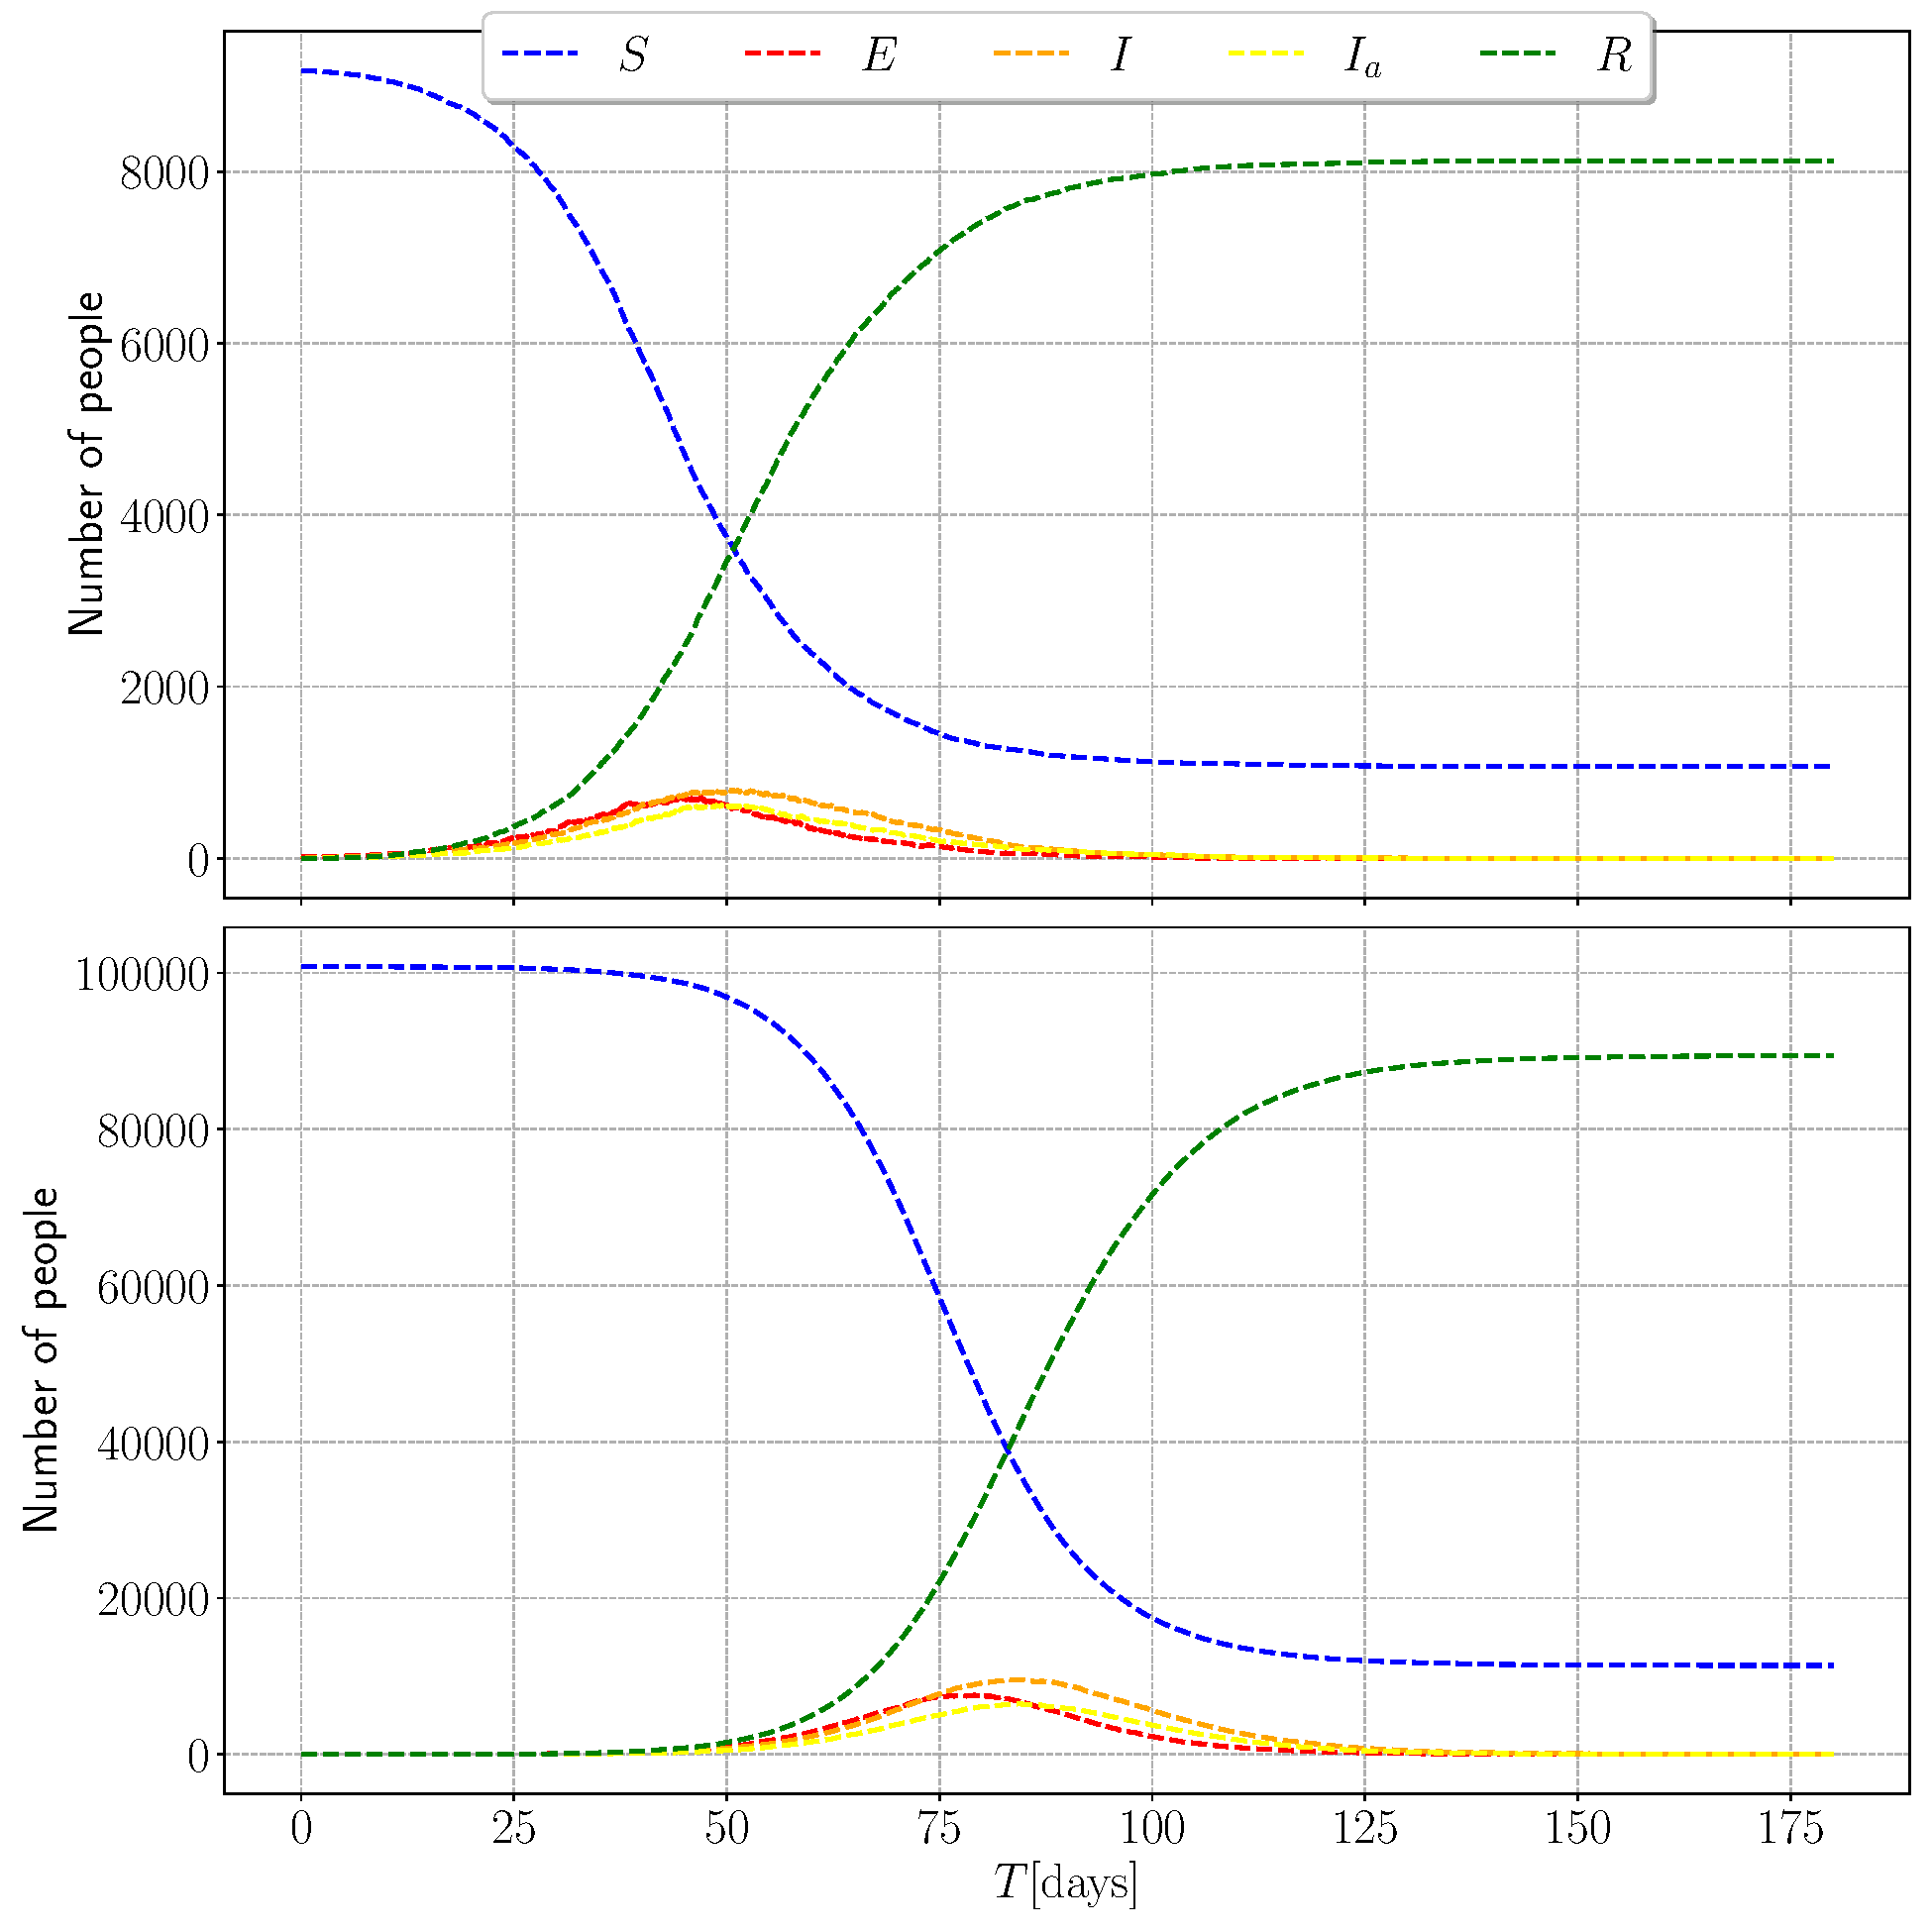
\includegraphics[width=0.8\columnwidth]{../fig/2Da_commuter.pdf}
	\caption{Solutions of Stochastic SEIIaR commuter model for the $2$-city case.}
	\label{fig:commuter_2city}
\end{figure}

\subsection{b) Description of implementation \& tests} 


To check that the system behaves as expected, we simulate the same scenario, only with another matrix which now represents \textit{no} flow of workers to the other areas:
\begin{equation}\label{eq:test_matrix}
	\mathbf{M} = \begin{bmatrix}
		10000 & 0 \\
		0 & 100000 
	\end{bmatrix}.
\end{equation}

The time-evolution of the different variables are shown in figure \ref{fig:test_commuter}, in which it is apparent that the exposed people in the small city never infect those in the large city, as we expect. The expected behaviour is also observed when the exposed start out in area $2$, but a plot of this is not included, for brevity. 


\begin{figure}[htb]
	\centering
	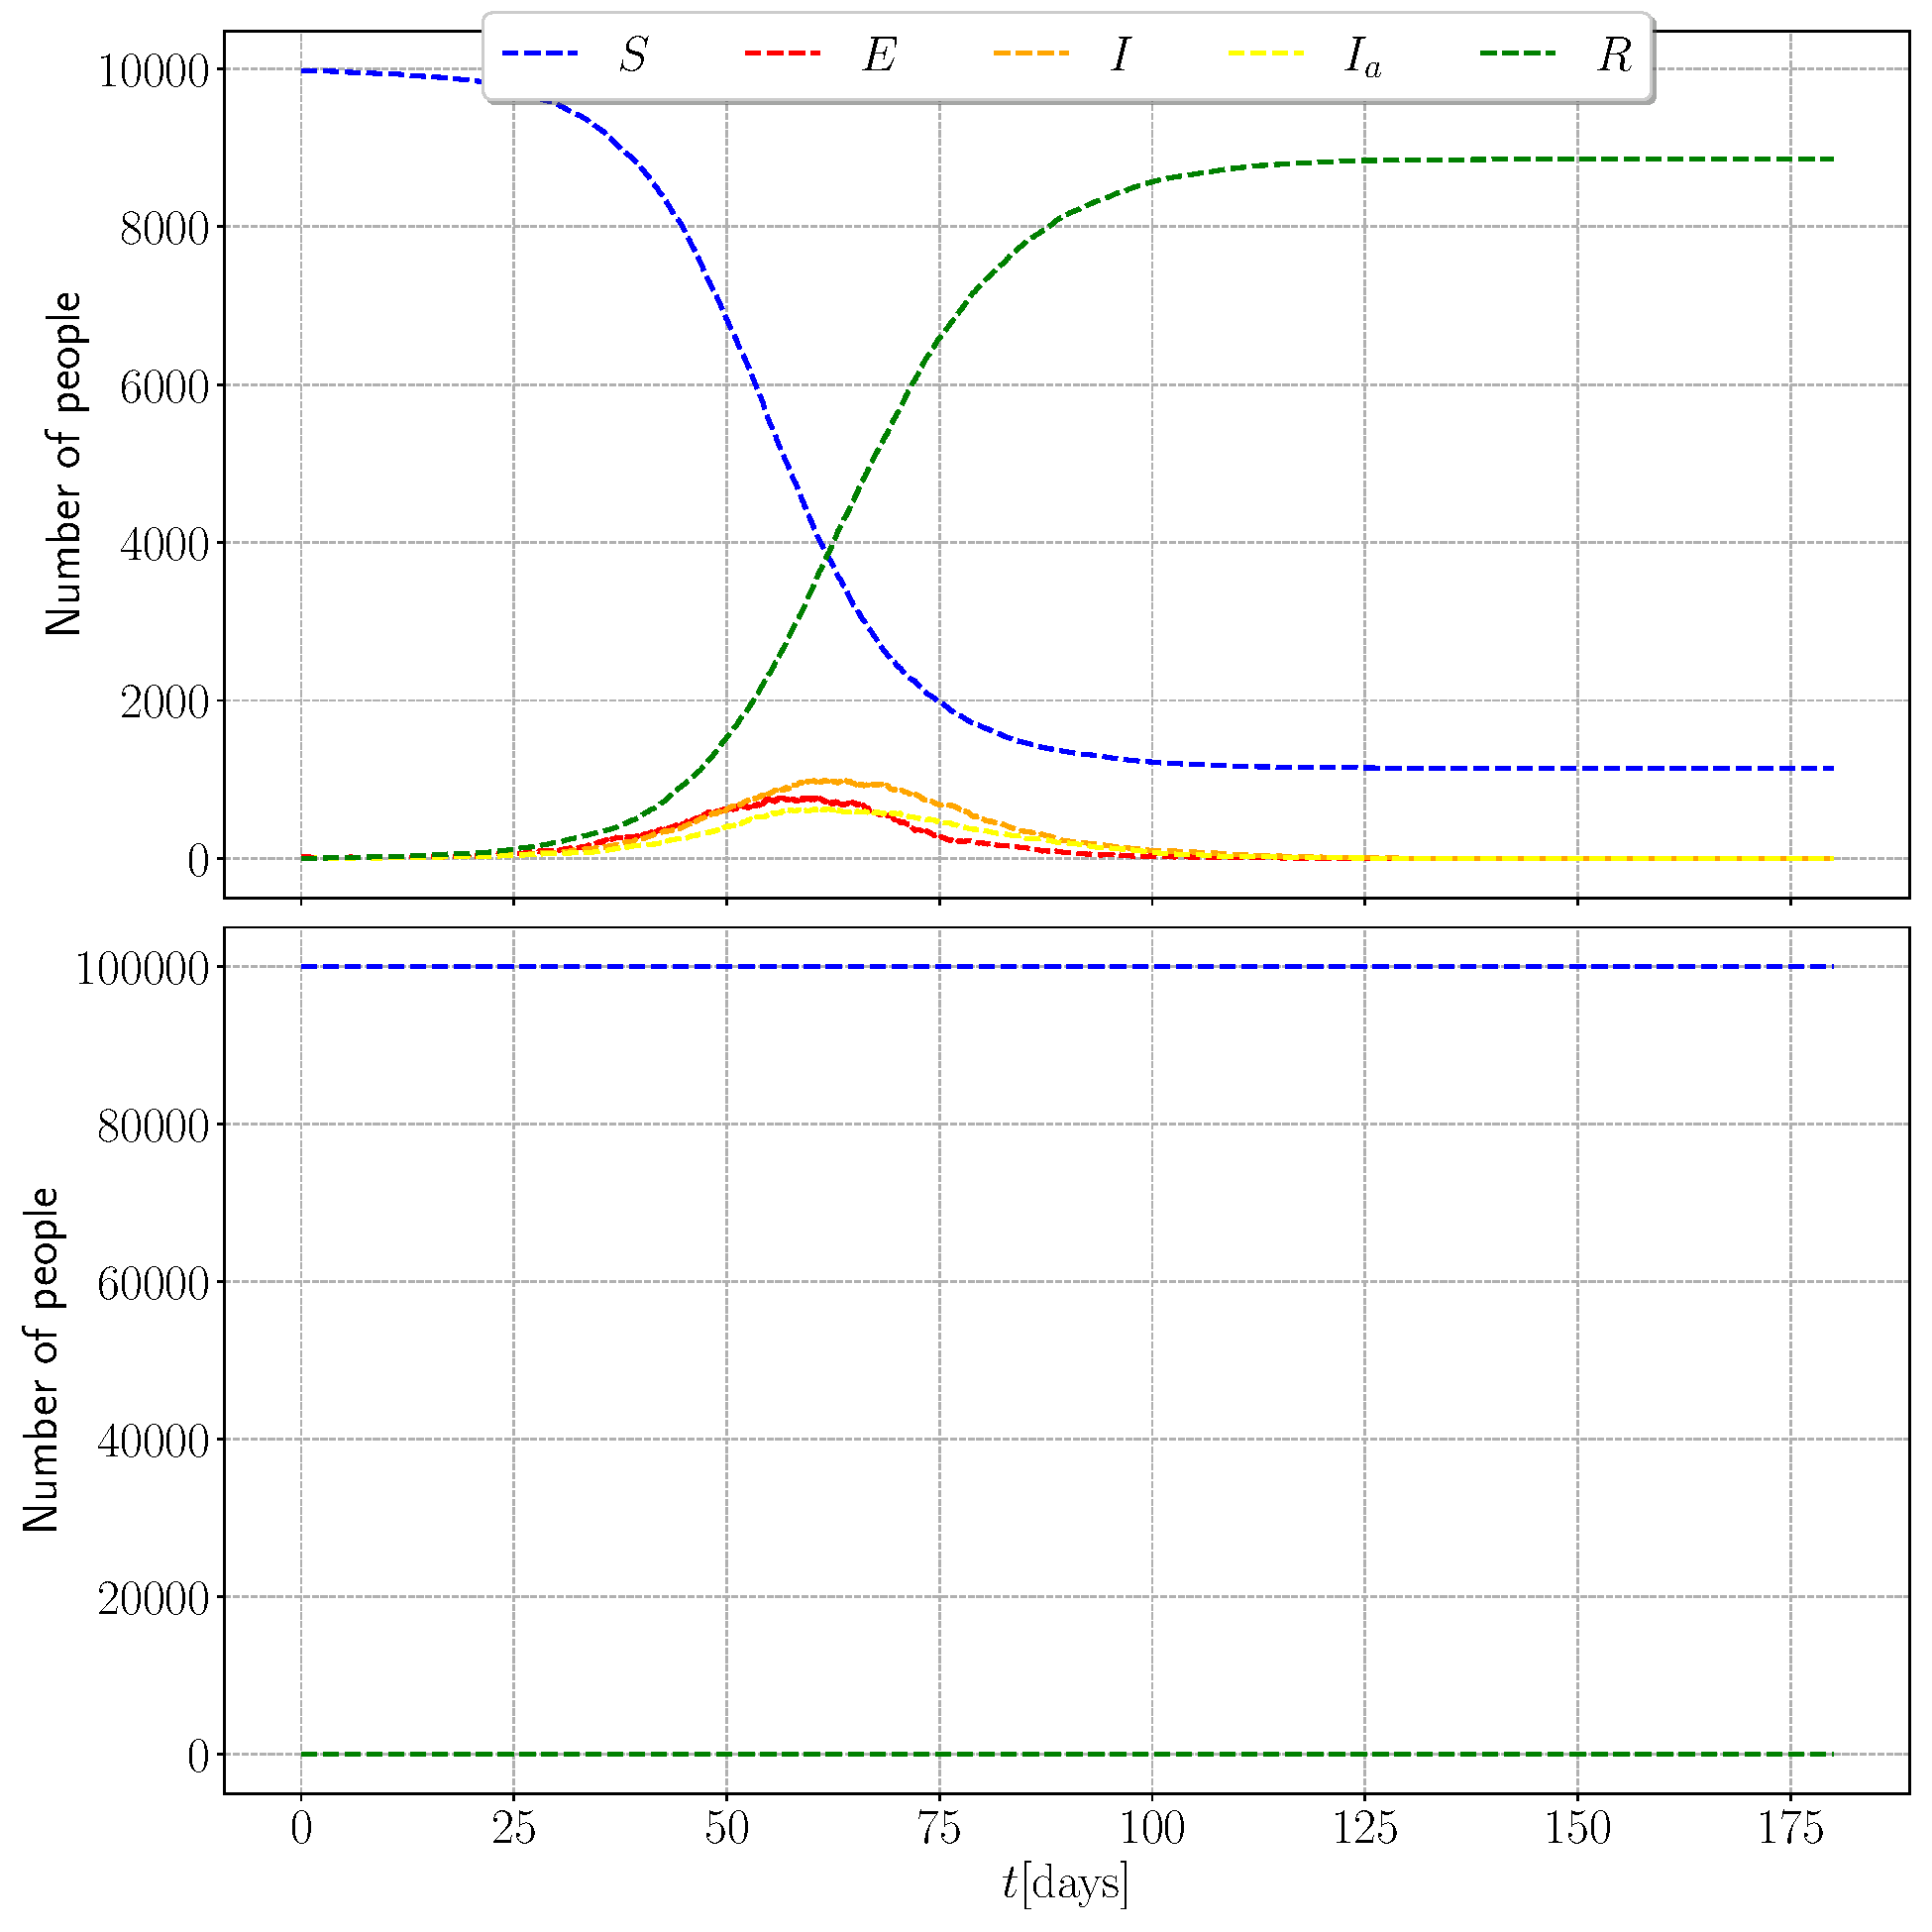
\includegraphics[width=0.8\columnwidth]{../fig/test_commuter.pdf}
	\caption{Solutions of Stochastic SEIIaR commuter model for the $2$-city case, with the matrix $\mathbf{M}$ in equation \eqref{eq:test_matrix}.}
	\label{fig:test_commuter}
\end{figure}